\subsubsection{22.11.14 (Соревнования)}
\begin{center}
	2-ый день соревнований "Робофест-Юг"
\end{center}
Сегодня проходили квалификационные матчи.
\newline 
Внесенные  доработки:
\begin{enumerate}
	\item Была написана программа для автономного периода: съезд с пандуса и забрасывание автономных мячей в 60-тисантиметровую корзину.
	\item Также было реализовано сбивание упора в одном из трех положений.
	\item На механизм захвата корзин были установлены откосы из стяжек для центровки захватываемой нами корзины. В дальнейшем планируется заменить стяжки  пластиковыми полосами, т.к. они часто ломаются.
	\begin{figure}[H]
		\begin{minipage}[h]{0.2\linewidth}
			\center  
		\end{minipage}
		\begin{minipage}[h]{0.6\linewidth}
			\center{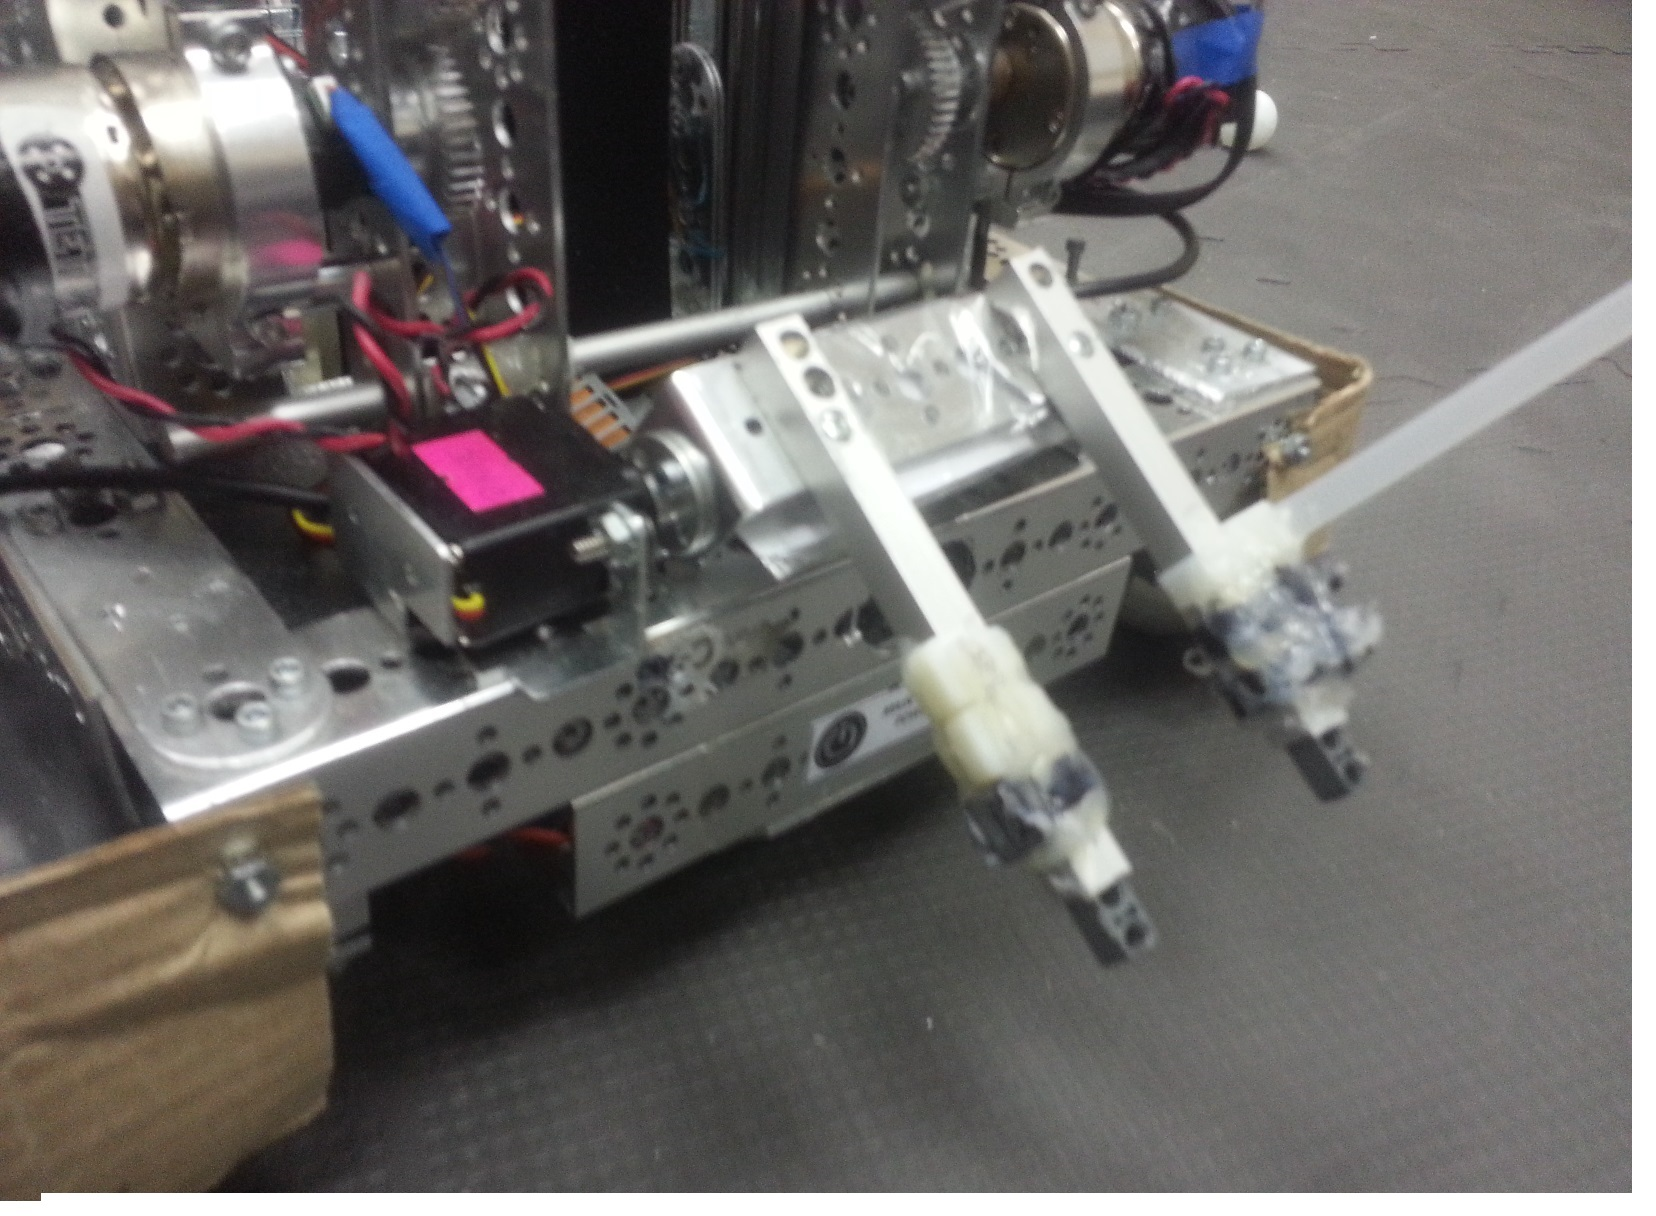
\includegraphics[scale=0.2]{days/22.11.14/images/01}}
			\caption{Откосы для центровки корзины.
			}
		\end{minipage}
	\end{figure}
	\item Во время одного из матчей у нашего робота сорвало NXT блок. Во избежание возникновения таких ситуаций в дальнейшем, NXT был дополнительно закреплен на резинки и закрыт балкой из набора Tetrix
	\begin{figure}[H]
		\begin{minipage}[h]{0.98\linewidth}
			\center{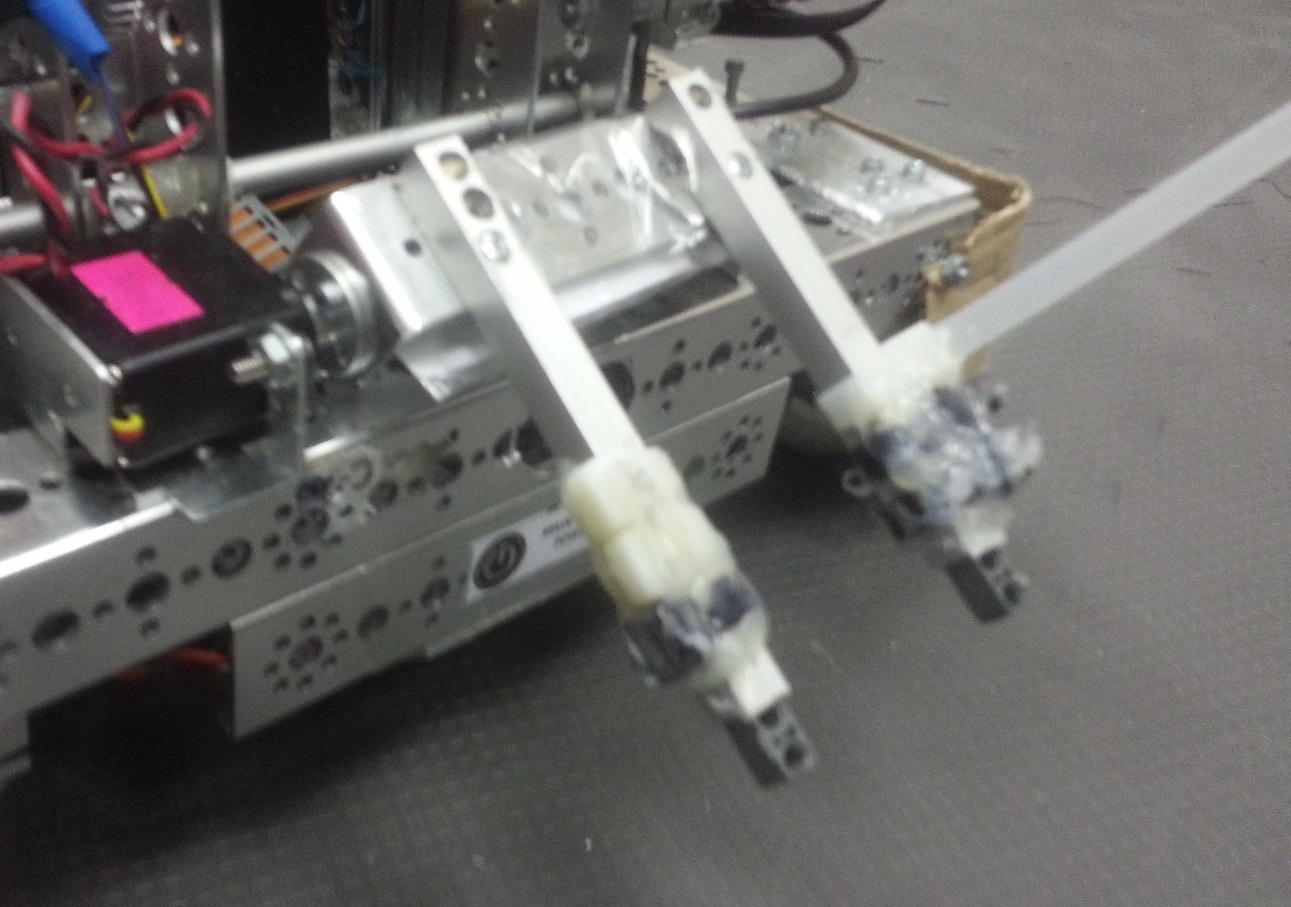
\includegraphics[scale=0.6]{days/22.11.14/images/02}}
		\end{minipage}
		\caption{Улучшенное крепление NXT}
	\end{figure}
	Результаты матчей: 2 победы из 4. 
	\newline
    Основные проблемы:
    \begin{enumerate}
       \item Неточное забрасывание мячей в передвижные корзины. Связано это с недостатком времени, уделенного тренировкам.
       \item Переодические перебои в работе сервопривода, опрокидывающего ковш, связаные с плохо закрепленным проводом и последующим его приходом в негодность.
    \end{enumerate} 
\end{enumerate}
\fillpage